\documentclass[a4paper]{article}

\usepackage[utf8]{inputenc}
\usepackage[portuguese]{babel}
\usepackage{a4wide}
\usepackage[pdftex]{hyperref}
\usepackage{graphicx}
\usepackage{wrapfig}

\begin{document}

\begin{titlepage}
\begin{center}


\includegraphics[width=0.6\textwidth]{logo}\\[1cm]

{\large Universidade do Minho - Escola de Engenharia}\\[0.5cm]

{\large Relatório do trabalho prático de POO}\\[0.5cm]

% Title
\rule{\linewidth}{0.5mm} \\[0.4cm]
{ \huge \bfseries UMeR \\[0.4cm] }
\rule{\linewidth}{0.5mm} \\[1.5cm]

% Author and supervisor
\noindent
\begin{minipage}{0.4\textwidth}
  \begin{flushleft} \large
    \emph{Autores :}\\
    Diana Costa \textsc{(A78985)}\\
    
\includegraphics[width=1.5cm]{diana}\break
    Marco Silva\textsc{(A79607)}\\
    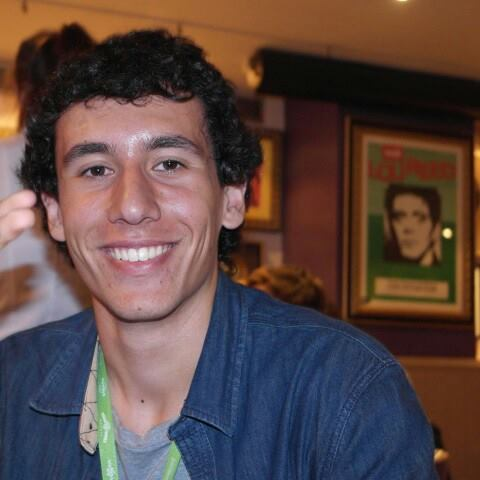
\includegraphics[width=1.5cm]{marco}\break
    Paulo Mendes\textsc{(A78203)}
    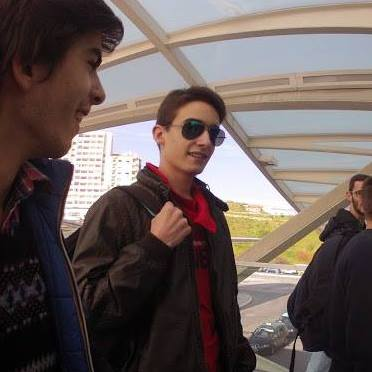
\includegraphics[width=1.5cm]{paulo}\break
  \end{flushleft}
\end{minipage}%
\begin{minipage}{0.4\textwidth}
  \begin{flushright} \large
    \emph{Grupo :} \\
    \textsc{nº 75}
  \end{flushright}
\end{minipage}

\vfill

% Bottom of the page
{\large Versão 1.0 \\ \today}

\end{center}
\end{titlepage}




\pagebreak
\begin{abstract}

\hspace{3mm} Perante a proposta para criar um serviço de transporte de passageiros - \emph{"UMeR"} - que permitisse um utilizador fazer viagens , houve um impasse inicial devido a necessidade de uma boa estruturação do problema. Tudo isto requeriu a escolha acertada, ou apropriada, das estruturas de dados a utilizar e da organização das diversas classes, de modo a que fossem aproveitadas todas as vantagens da implementação de um sistema de herança de classes.

Depois de algum tempo e trabalho, o resultado encontrado foi eficiente e satisfatório, e os objetivos e respostas às questões do enunciado proposto cumpridos.

\end{abstract}

\pagebreak
\tableofcontents

\pagebreak
\section{Introdução}
\label{sec:1}


\hspace{3mm} O projeto \emph{"UMeR"} surge no âmbito do projeto de Programação Orientada aos Objetos (POO), do Mestrado Integrado em Engenharia Informática da Universidade do Minho. Sendo um projeto de pequena/média dimensão a ser resolvido na linguagem \emph{Java}, este baseia-se na construção de um sistema que seja responsável por toda a gestão de uma empresa de taxis, quer ao nível das suas viaturas, funcionários(motoristas) e clientes.
\par Os utilizadores deste sistema(clientes) têm ao seu dispor algumas opções características numa empresa de táxis, nomeadamente a realização de viagens ou de requisição de uma viagem. Os motoristas, independentemente da empresa a que pertencem, tem à sua disposição um conjunto de viaturas que podem utilizar(conduzir), e serão sempre avaliados conforme o servido prestado ao cliente. Clientes e motoristas terão sempre um histórico de viagens realizadas numa determinada empresa. 
As viaturas podem ser de diversos tipos (carros, carrinhas de nove lugares, motos, ...), e têm associado, para além de um preço base por km e uma velocidade média por km, um fator de fiabilidade, que resulta da capacidade da viatura cumprir o tempo acordado com o cliente. Para além disso, algumas viaturas dispõe de uma fila de espera, para o caso de serem requisitadas por mais do que um cliente.
\par Assim sendo, houve a necessidade de pensar em estruturas e algoritmos para resolução dos métodos, explorando as potencialidades da linguagem \emph{Java}. Numa primeira fase, foi essencial o estudo das diversas bibliotecas do \emph{"Java 8"} como forma de aproveitamento de estruturas de dados e métodos associados.
\par Já no fim do projeto, a utilização do \emph{BlueJ} que vinha a ser feita desde o inicio do semestre facilitou  a execução de testes e resolução de erros.
\par Em suma, a Secção ~\ref{sec:2} descreve o problema a resolver, enquanto que a Secção ~\ref{sec:3} apresenta e discute a solução proposta pelo grupo, desenvolvida ao longo do semestre. Na secção ~\ref{sec:6} existe um manual de utilização da aplicação desenvolvida, e o relatório termina com conclusões, na  Secção ~\ref{sec:7}, onde é apresentada uma análise crítica dos resultados obtidos. Além disso, é feito um balanço tendo em conta as dificuldades ao longo do desenvolvimento do projeto.


\section{Descrição do Problema}
\label{sec:2}

\hspace{3mm} No contexto do projeto prático de POO, pode-se afirmar que foram propostas (ou necessárias) três tarefas. Como primeira instância, seria necessário estudar a API do \emph{"Java 8"}, como forma de decidir quais estruturas para armazenamento dos dados seriam mais convenientes. De seguida, seria necessário planear a estrutura do projeto em si, ou seja, como seriam divididas as classes, o que herdavam, se as estruturas de dados ficariam na própria empresa ou numa base de dados à parte, entre outros. Por fim, bastava implementar os métodos e permitir que todas as funcionalidades propostas no enunciado fossem cumpridas.
\par A primeira tarefa era de "simples" resolução, uma vez que todas as fichas resolvidas na unidade curricular ao longo do semestre facilitaram a compreensão de conceitos básicos de \emph{"Java"} e das potencialidades e adaptabilidade das diversas coleções.
\par Na segunda tarefa, foi necessário "sentar e pensar", isto é, todo o grupo reuniu-se para decidir como seria estruturado o trabalho, de acordo com os requisitos dos docentes no enunciado do trabalho prático. Exemplificando, seria necessário tomar decisões como "Que classes devemos "juntar" e de quais vão herdar dados?", "Que viaturas terão uma fila de espera, e qual o preço base por km de cada uma delas?", "Como será calculado o fator de fiabilidade de uma viatura, e como será implementada a questão do tempo real e tempo calculado?".
\par Já a terceira tarefa envolveu mais trabalho, dado que foi necessário implementar os métodos para resolver os requisitos do enunciado e testar se estariam a funcionar corretamente.


\section{Concepção da Solução}
\label{sec:3}

\hspace{3mm} Em grupo, foi proposto que, em conjunto, seriam resolvidas as grandes questões acerca da escolha e implementação da estrutura de dados a utilizar, bem como a estruturação de classes (super e sub classes). Numa segunda fase ocorreria a divisão das restantes tarefas pelos elementos do grupo, cada um responsável por implementar tudo o que é expectável numa classe.
\par Procurou-se assim obter uma linha de trabalho clara, eficaz e que permitisse obter os resultados expectáveis.


\subsection{Estruturas de Dados}
\label{sec:4}

\hspace{3mm} Foi essencial, para uma melhor compreensão de cada tarefa, definir de forma clara a estrutura de dados a adotar, pois a mesma pode ter um grande impacto no desenvolvimento das tarefas em si. Para isso foi necessário definir desde logo como tratar a informação passível de ser manipulada pelo programa.
\par Deste modo, e numa primeira fase, foi colocada a hipotese de utilização de \emph{ArrayLists}, pois seria de fácil utilização por parte dos elementos do grupo. Com a evolução do projeto e consequente resolução dos métodos para as diferentes classes e uma maior familiarização com a API, verificou-se que, já que a implementação da maioria destas seria baseada na procura de valores num array, o que implica um tempo médio de pesquisa de \emph{O(n)}, para a grande quantidade de dados propostos, ficaria aquém das expectativas, quando comparado com o tempo de procura apresentado por um HashMap, \emph{O(1)}. 
\par Assim sendo, já a meio da realização do projeto, foi decidido que a utilização de \emph{HashMaps} auxiliava a resolução dos métodos de uma forma mais eficiente, já que o tempo de procura de um elemento reduziria drasticamente. Esta estrutura de dados oferece vantagens praticamente em todo o projeto, já que a base deste é o acesso direto a Motoristas, Viaturas e Clientes.
\par Numa segunda fase, foram adicionados também estruturas para armazenamento do histórico de viagens já efetuadas (\emph{ArrayList}), e para a fila de espera dos veículos (\emph{HashMap}).
\par Em suma, por intermédio das estruturas de dados acima referidas, foi conseguida uma base sólida, e de fácil compreensão.



\subsection{Implementação}
\label{sec:5}

\hspace{3mm} Ao longo do projeto, as dificuldades encontradas foram bastantes e diversificadas.
Dado como clarificada a questão das API's e da escolha das estruturas de dados, resta falar da implementação de métodos necessários para o funcionamento do projeto. Tendo como primeiro foco a estruturação das classes, foi necessária alguma reflexão sobre este ponto devido às várias hipoteses de implementações, e da melhor maneira possível, para  que fossem aproveitadas certas vantagens, e depois fazer o balanço final da melhor solução. Os principais pontos alvos de análise foram a reutilização de código, quer por herança quer por composição, e vendo em cada um dos casos qual seria a melhor solução, não só a nível de eficiencia, como também se a relação em si faria sentido (como foi abordado nas aulas práticas).
\par Dentro do mesmo tema (implementação de métodos), é também de salientar a importância do estabelecimento de classes abstratas na implementação do projeto como forma de "obrigação" de definição de determinados métodos essenciais. Uma grande interrogação que surgiu entre o grupo de trabalho foi relativo a uma viatura poder ter uma fila de espera, em que nessa fila estariam os clientes que requisitaram uma viatura específica, quando esta não estava disponível. Na hipotese de cada uma das viaturas permitir fila de espera, a \emph{"queue"} poderia estar efetivamente na classe da viatura, mas esta seria uma solução que não respeitaria o princípio da reutilização de código o que levou a criar uma variável em cada viatura \emph{"hasQueue"}, que permite saber se uma viatura tem a capacidade de ter fila de espera, e na classe "Empresa" estaria uma coleção que reunia as viaturas que possuem esta característica. Na seguinte imagem está a arquitetura final das classes.

\begin{figure}[htp]
\centering
\includegraphics[width=12cm]{classes}
\caption{Arquitetura final das classes}
\label{fig:classes}
\end{figure}

\pagebreak
\par Outro ponto de discussão foi a questão da implementação da interface. Tendo em conta o tempo definido para cada classe, a interface foi, sem dúvida, a mais demorada e de maior escala, devido à  complexidade desta tarefa e a compreensão a fundo do enunciado.
\par Mudando de tema, agora para a questão da serialização, foram também encontradas dificuldades, principalmente devido ao raciocínio que este processo implica. Foram discutidas várias possibilidades de serialização, nomeadamente quais seriam os dados essenciais para uma recuperação completa de um estado do projeto, que tivesse sido anteriormente interrompido. Disto derivou a seguinte questão: "Guarda-se o programa como um todo, ou divide-se por ficheiros informações diferentes?". Depois de falar com os docentes, decidiu-se então que a empresa seria guardada como um todo.
\par Um último problema baseava-se no facto de como seria calculado o tempo real e o tempo teórico, acordado entre motorista e cliente, que teria penalizações ou benefícios para a viatura e o motorista. Isto foi conseguido atráves do cálculo do preço teórico (com base no preço teórico por quilometro da viatura em questão) e o cálculo da distância entre a posição atual do cliente e o destino pretendido. Neste cálculo é considerado também um valor aleatório representativo de factores que podem provocar atrasos nos serviços prestados pelo taxista.
\par Generalizando e finalizando, uma das grandes tarefas realizadas e que se revelou complexa foi a correção de erros resultante da interligação entre classes, redefinição e herança de métodos, e implementação de construtores, utilizando os construtores de super-classe (\emph{super()}). Conseguiu-se assim a criação de uma linha de trabalho clara durante a execução do projeto.

\pagebreak
\section{Manual de utilização da aplicação}
\label{sec:6}

\begin{wrapfigure}{l}{0.25\textwidth}
\includegraphics[width=0.9\linewidth]{logumer} 
\caption{Logótipo da UMeR}
\label{fig:logumer}
\end{wrapfigure}

\hspace{3mm} A aplicação desenvolvida "UMeR" tem como principal alvo (num contexto real) empresas de táxi que pretendam gerir a sua empresa e funcionários, e respetivos clientes que queiram requesitar um transporte. As "regras" de utilização da aplicação, tais como as suas explicações, vão seguir um contexto académico, e responder aos requesitos do enunciado prático deste projeto.
\par No ecrã inicial da aplicação, pode-se encontrar a opção de carregar, ou não, os dados de um ficheiro correspondente a um estado da aplicação já existente. Caso o utilizador decida carregar, terá de inserir o nome do ficheiro e será redireccionado para a sua empresa já criada. Caso pretenda "criar" uma empresa nova, deverá introduzir "0", como é sugerido no ecrã.
\par De seguida, aparece o ecrã inicial da "UMeR" com a saudação "Bem Vindo à UMeR". Aqui é possível criar empresas (opção "Criar Nova Empresa") ou, depois de criadas, gerir a que o utilizador quiser (opção "Carregar Empresa"). Dever-se-á primeiro criar uma empresa, atribuindo-lhe um nome como é sugerido, e depois a empresa será adicionada à base de dados do sistema. De seguida, será reencaminhado de volta ao ecrã principal, e poderá criar mais empresas ou carregar a empresa acabada de criar.
\par Após o utilizador carregar a empresa que acabara de criar, será encaminhado para um ecrã inicial da sua empresa com a saudação "Bem vindo à (nome Empresa) !". Aí terá diversas opções, entre elas, "Registar Nova Conta". No contexto de uma empresa acabada de criar, esta será a opção a escolher, e a partir daqui são registados clientes ou motoristas. Assim, depois do utilizador escolher registar uma nova conta e se selecionar cliente, ser-lhe-ão pedidos nome, email, password, morada, data de nascimento e coordenadas atuais (x e y), e ser-lhe-á mostrado uma mensagem temporária com os dados que inseriu. Caso tenha selecionado um motorista, os dados pedidos são os mesmos que o cliente, exceto as coordenadas, e será automático o estado de "está a trabalhar".
\par Depois de registadas as contas, a próxima opção a escolher deverá ser "Adicionar Veículo", e selecionar o tipo de veículo de acordo com os sugeridos no ecrã (carro, carrinha de 9 lugares, moto ou bicicleta). Em qualquer dos veículos, vai ser pedido a matrícula do mesmo, a sua velocidade média, o preço por quilómetro, fator de fiabilidade e coordenadas (x e y). Por fim, o utilizador escolhe se o veículo que está a criar vai possuir ou nao fila de espera. No fim, aparecerá um ecrã temporário com os dados do veículo acabado de criar.
\par O próximo passo será "Associar Motorista a Veículo", que permite interligar os motoristas aos táxis que vão passar a conduzir. Será necessário apenas introduzir o email do motorista e a matrícula do táxi (identificadores de motorista e veículo).
\par Passando para a opção "Iniciar Sessão", é apenas válida para os clientes, e pede para serem inseridos o email e palavra passe dos últimos. De seguida, surgem as opções de pedir um "Táxi mais próximo" ou um "Taxi específico". No caso do táxi mais próximo, serão pedidas as coordenadas (x e y) para onde o cliente pretende ir, a viagem é efetuada, e é pedida uma classificação da viagem. No caso  de ser solicitado um taxi específico, é pedido o email do motorista que se pretende requisitar e as coordenadas do destino (x e y).
\par Por fim, resta a opção de "Guardar" a empresa atual, onde é assegurada toda a informação inserida no sistema.
\par Para sair da aplicação, o utilizador deve premir "Sair".

\pagebreak
\section{Conclusões}
\label{sec:7}

\hspace{3mm} Tendo em conta o objetivo do projeto, a criação de um sistema que permitisse a realização de viagens foi de facto um projeto interessante e desafiante para todos os elementos do grupo. A implementação deste sistema permitiu não só o desenvolvimento das capacidades de raciocínio e programação dos alunos, mas também foi como um primeiro contacto com o que será o futuro dos mesmos, a nível do uso de API's e manuseamento de trabalho e implementações já existentes.
\par De facto, o maior obstáculo deste projeto, ao contrário das unidades curriculares anteriores, foi o estudo de diversas bibliotecas, e a obtenção de uma linha de raciocínio que tivesse em conta o desenvolvimento de uma "semi-aplicação", que, na vida real, poderia servir para gerir uma empresa de táxis. Todo o esforço feito na escolha das estruturas de dados permitiria uma resolução simples e eficaz dos \emph{métodos} propostos, baseadas em iterações por estruturas de dados à procura da informação pretendida, por exemplo, e extrapolando para um contexto real, por um veiculo específico a ser requerido por um cliente.
\par Por último, o resultado foi extremamente positivo. A implementação deste sistema foi conseguida com sucesso e o trabalho de semanas por fim deu frutos.

\end{document}